%!TEX root = ..\lections.tex
На первой лекции мы уже сталкивались с понятием точечного
отображения. Продолжим знакомство с этим важным и удивительным
объектом нелинейной динамики. Можно выделить два основных сценария
возникновения моделей в виде точечных отображений. Во-первых, для многих
реальных систем характерно изменение их состояний лишь в некоторые
моменты времени. Ясно, что наиболее адекватное описание поведения таких
систем можно получить с помощью моделей с дискретным временем и, в
частности, моделей в форме точечных отображений. Во-вторых, точечные
отображения могут порождаться траекториями динамических систем с
непрерывным временем.

\section{Точечные отображения -- модели дискретных систем}%
\label{sec:6.1}

В настоящее время для управления самыми различными объектами и
процессами широкое распространение получили цифровые автоматические
системы. Такие системы оперируют цифровыми кодами, получаемыми из
непрерывных сигналов путем их квантования по уровню и времени. В
частности, в радиоавтоматике, связи, телевизионных системах,
радиоизмерительных устройствах используются импульсно-фазовые системы
автоподстройки частоты (ИФАП). Как и непрерывная система фазовой
автоподстройки частоты (см. \ref{lect4}), система ИФАП содержит кольцо
авторегулирования. Однако в кольце обратной связи системы ИФАП
используется информация об ошибке, взятая в отдельные моменты времени.
Для этого в типовую структуру схемы ФАП (рис. \ref{fig:4.10}) вводятся
дополнительные элементы: формирующее устройство, преобразующее
синусоидальные сигналы генераторов в короткие импульсы, запоминающее
устройство, фиксирующее выходное напряжение фазового детектора, который
является импульсным, в промежутке между соседними импульсами. Типовая
система ИФАП с идеальным запоминанием и отсутствием фильтра в цепи
управления описывается уравнением
\begin{equation}
        \label{eq:6.1}
        \phi(n+1) - \phi(n) + \alpha F( \phi(n)) = \gamma.
\end{equation}
Уравнение \eqref{eq:6.1} связывает разность фаз $\phi$ сигнала подстраиваемого генератора
и опорного сигнала в соседние моменты времени $n$ и $n+1$, где $n = 1,2,3,\dots$
соответствует моментам времени $t=n \tau_0$, а $\tau_0$--период дискретизации.
В \eqref{eq:6.1} $F( \phi)$-- $2 \pi$-периодическая функция --
 характеристика фазового дискриминатора,
нормированная на единицу,
$\gamma = \Omega_H \tau_0$
-- параметр пропорциональный
начальной расстройке
$\Omega_H$ генераторов, $\alpha = \Omega \tau_0$
-- параметр цепи управления.
В силу инвариантности уравнения \eqref{eq:6.1} относительно преобразования
$\phi \to \phi + 2 \pi$ , оно представляет собой точечное отображение окружности на
себя.

Другими примерами реальных процессов, которые адекватно
описываются точечными отображениями, могут служить колебания
численности биологических популяций. Например, динамика некоторых
популяций в замкнутой среде достаточно хорошо описывается (П.Ф.
Ферхюльстом, 1845) так называемым логистическим отображением
\begin{equation}
        \label{eq:6.2}
        x(n+1) = \mu x(n) (1- x(n)),
\end{equation}
где $x(n)$ -- нормированная численность особей в $n$-й год, а $\mu$ -- параметр, зависящий от плодовитости особой
в $(n+1)$-й год -- $x(n+1)$ пропорциональна численности в предыдущий год --
$x(n)$ и свободной части жизненного пространства, которая в свою очередь пропорциональная величине $(1 - x(n))$.

\section{Отображение Пуанкаре}%
\label{sec:6.2}

Как мы уже отмечали,  в некоторых случаях точечные отображения могут
генерироваться траекториями динамических систем с непрерывным временем.
Такие отображения называют \textbf{отображениями Пуанкаре} . Поясным процедуру
возникновения отображения Пуанкаре на простейшем примере. Рассмотрим
систему с непрерывным временем вида
\begin{equation}
        \label{eq:6.3}
        \begin{cases}
                \dot x = y,
                \dot y = -2 \delta y - \omega_0^2 x,
        \end{cases}
\end{equation}
где $\delta$ и $\omega_0$--положительные параметры. 
Система \eqref{eq:6.3} описывает динамику
линейного осциллятора с диссипацией (см. \ref{lect5}). Пусть $\omega_0^2>\delta^2$ . В этом
случае на фазовой плоскости системы \eqref{eq:6.3} существует единственное
устойчивое состояние равновесия в начале координат -- устойчивый фокус,
который притягивает все остальные траектории системы (рис. \ref{fig:6.1}а). Покажем,
что траектории системы \eqref{eq:6.3} порождают одномерное точечное отображение
полупрямой $N = \qty{y=0, ~ x<0}$ на себя. Запишем общее решение системы \eqref{eq:6.3}
\begin{equation}
        \label{eq:6.4}
        \begin{cases}
                x(t) = e^{-\delta t} \qty[ C_1 \cos(\omega t) + C_2 \sin(\omega t) ],\\
                y(t) = e^{-\delta t} \qty[ (C_2 \omega - \delta C_1) \cos(\omega t) - (C_2 \delta + C_1 \omega) \sin( \omega t) ],  
        \end{cases}
\end{equation}
где $\omega = \sqrt{ \omega_0^2 - \delta ^2}$, $C^{1,2}$ -- произвольные константы. Рассмотрим траекторию $L$,
выходящую при $t=0$ из некоторой произвольной точки с координатами $x=x_{0}$ 
$(x_0>0)$, $y=0$ (см. рис.\ref{fig:6.1}а). Из \eqref{eq:6.4} получаем уравнение траектории $L$ 
\begin{equation}
        \label{eq:6.5}
        \begin{cases}
                x(t) = e^{-\delta t} x_0 \qty[ \cos(\omega t) + \frac{\delta}{\omega} \sin(\omega t) ],
                y(t) = e^{- \delta t} x_0 \qty( \frac{\delta^2}{\omega} + \omega)   \sin(\omega t).
        \end{cases}
\end{equation}

\begin{figure}[h]
        \centering
        \begin{minipage}{0.49\linewidth}
                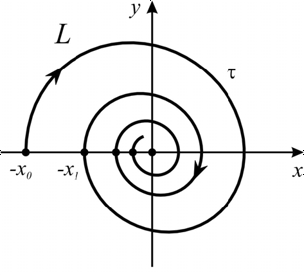
\includegraphics[width=\linewidth]{fig/lect6/1a}
        \end{minipage}
        \begin{minipage}{0.49\linewidth}
                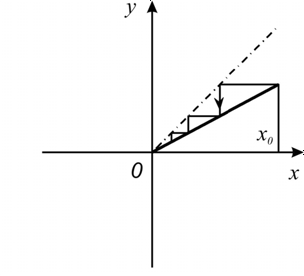
\includegraphics[width=\linewidth]{fig/lect6/1b}
        \end{minipage}
        \caption{Фазовый портрет системы \eqref{eq:6.3} (а); отображение Пуанкаре \eqref{eq:6.8} (b).}
        \label{fig:6.1}
\end{figure}
Найдём координату точки, в которой $L$ первый раз пересекает полупрямую $N$. Обозначим через $\tau$ время движения по траектории $L$ между этой и начальной точками. Тогда координаты искомой точки можно найти из условий
\begin{equation}
        \label{eq:6.6}
        y(\tau) = 0, \quad x(\tau) = - x_1.
\end{equation}
Из \eqref{eq:6.6}, используя \eqref{eq:6.5}, получаем
\begin{equation}
        \label{eq:6.7}
        \tau = \frac{2 \pi}{\omega} \text{ и } x_1 = e^{-\delta \frac{2 \pi}{\omega}} x_0. 
\end{equation}
Поскольку точка $x_0$ была произвольной, уравнение \eqref{eq:6.7} задает преобразование любой точки полупрямой $N$, т.е. искомое точечное отображение
\begin{equation}
        \label{eq:6.8}
        \bar x = e^{- \delta \frac{ 2 \pi}{\omega}} x.
\end{equation}
Отображение \eqref{eq:6.8} – линейное точечное отображение. Качественный вид
отображения представлен на рис. \ref{fig:6.1}b. Его динамика чрезвычайно проста –
любая траектория отображения асимптотически приближается к значению $x=0$.
Прямая $N$, на которой определено отображение Пуанкаре, называется \textbf{секущей
Пуанкаре} (термин <<секущая>> отражает наличие потока траекторий,
проходящего через нее).

Рассмотренный пример показывает, что для секущей Пуанкаре характерны следующие свойства
\begin{itemize}
        \item возвращаемость траекторий;
        \item во всех точках траекторий пресекают секущую так, что наклон касательных к ним в этих точках не равен нулю (такое пересечение называется трансверсальным см. лекцию \ref{lect1}.
\end{itemize}
Заметим, что секущей Пуанкаре может быть не обязательно прямая, а,
например, некоторая кривая (для систем на плоскости), на которой
выполняются вышеперечисленные свойства. Очевидно, что в общем случае
размерность секущей Пуанкаре на единицу меньше размерности фазового
пространства динамической системы. Например, для систем с трехмерным
фазовым пространством это двумерная поверхность. Секущая Пуанкаре может
быть как локальной, когда ее пересекает лишь часть траекторий, так и
глобальной, когда ее пересекают все траектории динамической системы
(например, как в случае системы \eqref{eq:6.3}). Заметим также, что отображение
Пуанкаре существует далеко не всегда. Например, если на фазовой плоскости
существует единственное состояние равновесия \textbf{седло} , с сепаратрисами,
уходящими в бесконечность, то отображение Пуанкаре не существует.

Однако, существует важный класс динамических систем, для которого
секущая Пуанкаре всегда существует и, более того, является глобальной. Это
неавтономные системы с периодической правой частью (например, системы,
находящиеся под действием периодического внешнего силового воздействия).
Поясним ситуацию на примере неавтономной системы второго порядка
\begin{equation}
        \label{eq:6.9}
        \begin{cases}
                \dot x_1 = f_1 (x_1,x_2,t) \\
                \dot x_2 = f_2 (x_1,x_2,t), 
        \end{cases}
\end{equation}
где $f_i(x_1,x_2,t)$-- периодические функции с периодом $T = \frac{2 \pi}{\omega}.$ Сделав в \eqref{eq:6.9} замену $t = \frac{\theta}{\omega}$, получим систему
\begin{equation}
        \label{eq:6.10}
        \begin{cases}
                \dot x_1 = f_1 \qty( x_1,x_2, \frac{\theta}{\omega}),\\
                \dot x_2 = f_2 \qty(x_1,x_2, \frac{\theta}{\omega}), \\
                \dot \theta = \omega.\\
        \end{cases}
\end{equation}
Система \eqref{eq:6.10} -- автономная система третьего порядка, не имеющая
состояний равновесия в силу того, что $\dot \theta = \omega>0$. Отсюда также следует, что люьая траектория системы \eqref{eq:6.9}, <<стартующая>> с плоскости 
$\Sigma = \qty{ t =t_0=\const, ~ ( x_1,x_2) \in \R^2}$, за конечное время придёт на плоскость
$\Sigma = \qty{ t=t_0 + \frac{2\pi}{\omega}, ~ (x_1,x_2) \in \R^2}$ (см. рис.\ref{fig:6.2}).
\begin{figure}[h]
        \centering
        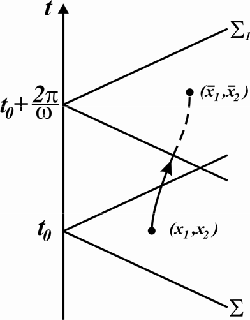
\includegraphics[]{fig/lect6/2}
        \caption{Генерация отображения Пуанкаре системой \eqref{eq:6.9}}
        \label{fig:6.2}
\end{figure}
В силу периодичности правых частей системы \eqref{eq:6.9} плоскости
$\Sigma$ и $\Sigma_1$ тождественны и, следовательно, систему \eqref{eq:6.9} порождает двумерное точечное отображение
\begin{equation}
        \label{eq:}
        P: \quad \Sigma \to \Sigma.
\end{equation}

Конечно, рассмотренный выше простейший пример (система \eqref{eq:6.3})
введения отображения Пуанкаре не позволяет в полной мере судить о
целесообразности такой процедуры. Однако, позднее на более содержательных
примерах мы покажем, что исследование динамических систем с помощью
отображения Пуанкаре является одним из эффективных методов современной теории колебаний.

Перейдем к изучению свойств точечных отображений.

\section{Неподвижные точки}%
\label{sec:6.3}

Рассмотрим $m$-мерное нелинейное точечное отображение
\begin{equation}
        \label{eq:6.11}
        \bar{ \vec x} = \vec F(\vec x), ~ \vec x \in \R^m, ~ \vec F: \R^m \to \R^m.
\end{equation}
Напомним, что в \eqref{eq:6.11} $ \bar{\vec x} = \vec x (n+1)$, а  $\vec x \equiv \vec x(n)$, а $n$-- дискретное время. Аналогично случаю динамических систем с непрерывным временем, для системы \eqref{eq:6.11} также можно ввести понятие полутраектории и траектории, которые задаются соответственно следующим образом
\begin{equation}
        \label{eq:}
        \qty{ \vec F^n \vec x_0}_{n=0}^{+\infty}
        \text{ и }
        \qty{ \vec F^n \vec x_0}_{n=-\infty}^{+\infty},
\end{equation}
где $\vec x_0 = \vec x(0)$. Очевидно, что в фазовом пространстве системы \eqref{eq:6.11}
они
представляют собой последовательности точек. Простейшим видом траекторий
системы  \eqref{eq:6.11} являются так называемые неподвижные точки. Неподвижными
точками отображения  \eqref{eq:6.11} называются такие значения $x$ , которые не
изменяются под его действием, т.е. являются решениями системы
\begin{equation}
        \label{eq:6.12}
        \vec x = \vec F( \vec x).
\end{equation}
Пусть $\vec x = \vec x^*$ -- решение системы  \eqref{eq:6.12} и, следовательно, $\vec x = \vec x^*$ --
одна из неподвижных точек отображения  \eqref{eq:6.11}. Для неподвижных точек, аналогично состояниям равновесия
конечномерных систем с непрерывным временем
может быть введено понятие устойчивости по Ляпунову. Незначительное
различие состоит в дискретности времени и траекторий, Далее, говоря об
устойчивости неподвижных точек, мы будем понимать их устойчивость в
смысле Ляпунова. Запишем отображение \eqref{eq:6.11} в новых переменных
\begin{equation}
        \label{eq:6.13}
        \vec \xi = \vec x - \vec x^*
\end{equation}
Из \eqref{eq:6.11} и \eqref{eq:6.13} имеем
\begin{equation}
        \label{eq:6.14}
        \vec x^* + \bar{ \vec \xi} = \vec F \qty( \vec x^* + \vec \xi).
\end{equation}
Разлагая правые части системы \eqref{eq:6.14} в степенные ряды по $\vec \xi$, приходим к линейному 
$m$-мерному отображению
\begin{equation}
        \label{eq:6.16}
        \bar{\vec{\xi}} = \vec A \vec{\xi},
\end{equation}
где $\vec A$--постоянная $m \times m$-матрица с элементами $\displaystyle a_{ik} = \pdv{f_i}{x_k} \eval_{x=x^*}$. Будем искать решение системы \eqref{eq:6.16} в виде
\begin{equation}
        \label{eq:6.17}
        \vec{\xi}(n) = \vec C (s)^n,
\end{equation}
где $\vec C$ -- постоянный вектор столбец. Подставляя \eqref{eq:6.17} в \eqref{eq:6.16}, получим характеристический определитель
\begin{equation}
        \label{eq:6.18}
        \det(\vec A - s \vec E) = 0,
\end{equation}
где $\vec E$-- единичная $m \times m$-матрица. Раскрывая определитель \eqref{eq:6.18}, приводим к характеристическому уравнению. Корни этого уравнения, которые обозначим через $s_{i},~ i=1,2,\dots,m,$ называются \textbf{мультипликаторами} неподвижной точки $\vec x = \vec x^*$.

На предыдущей лекции мы отмечали, что структура траекторий в
окрестности грубого состояния равновесия топологически эквивалентна ее
линеаризации. Аналогичное утверждение справедливо и для неподвижных
точек. Именно, если мультипликаторы неподвижной точки удовлетворяют
условию  $|s_i| \neq 1,~ i=1,2,\dots,m,$, то она является грубой (структурно устойчивой) и
существует гомеоморфизм, который переводит каждую траекторию из
достаточно малой окрестности неподвижной точки нелинейного отображения
\eqref{eq:6.11} в траекторию из окрестности соответствующей неподвижной точки
линейного отображения \eqref{eq:6.16} с сохранением направления движения.
Следовательно, грубые неподвижные точки отображения \eqref{eq:6.11} могут быть
исследованы на устойчивость и классифицированы с помощью
соответствующих линейных отображений. В частности, из \eqref{eq:6.17} следует, что
неподвижная точка
$\vec x = \vec x^*$ отображения \eqref{eq:6.11} будет асимптотически
устойчивой $n \to + \infty$ , если все ее мультипликаторы
$s_i$ 
 на комплексной
плоскости лежат строго внутри единичной окружности, т.е. удовлетворяют
условию
\begin{equation}
        \label{eq:6.19}
        |s_i| < 1, i = 1,2,\dots,m.
\end{equation}
Если же среди мультипликаторов $s_i$ существует хотя бы один расположенный на комплексной плоскости вне единичной окружности, то неподвижная точка $\vec x = \vec x^*$ отображения \eqref{eq:6.11} неустойчива по Ляпунову.

\section{Одномерные линейные отображения}%
\label{sec:6.4}

Рассмотрим отображения \eqref{eq:6.16} в одномерном $(m=1)$ случае 
\begin{equation}
        \label{eq:6.20}
        \bar{\xi} = a \xi, 
\end{equation}
где $a$- параметр, $a\neq 0$. Предположим сначала, что $a \neq 1$. Очевидно, что $\xi=0$--
неподвижная точка отображения \eqref{eq:6.20}. Будем искать решение уравнения \eqref{eq:6.20} в виде \eqref{eq:6.17}. Подставляя \eqref{eq:6.17} в \eqref{eq:6.20} находим, что мультипликатор $s = a$. Следовательно, неподвижная точка $\xi=0$ является асимптотически устойчивой, если
$|a|<1$ и неустойчивой, если $|a|>1$.

Рассмотрим как переменная $\xi(n)$ изменяется во времени $n$ под действием отображения \eqref{eq:6.20} при различных значениях параметра.

В случае одномерных отображений (отображение \eqref{eq:6.11} в случае $m=1$ ) и, в частности, отображения \eqref{eq:6.20}, эволюцию $\xi(n)$ удобно изучать с помощью так называемой 
\textbf{диаграммы Ламерея}. 
 Отображение рассматривается не в фазовом
пространстве, которое является одномерным, а на вспомогательной плоскости
$(x,\bar x)$. На этой плоскости каждой траектории отображения соответствует
некоторая ломаная линия, которая строится следующим образом. Прежде всего,
на плоскости $(x,\bar x)$ проводится построение графика функции $F(x)$, которую
называют \textbf{функцией последования}. При этом точки пересечения этого графика
с биссектрисой $\bar x = x$ соответствуют неподвижным точкам отображения. Затем
из точки на оси абсцисс, соответствующей начальному условию
$x_0$,
несовпадающему с координатами неподвижных точек, проводится
вертикальная прямая до пересечения с графиком функции последования $F(x)$ .
Ордината найденной таким образом точки соответствует значению 
$x(1) = F(x_0)$.
Далее из этой точки проводится горизонтальная прямая до пересечения с
биссектрисой. Тем самым устанавливается новая начальная точка на оси
абсцисс для нахождения следующей итерации отображения, т.е.  $x(2)=F(x(1))$ .
Затем процедура повторяется и на плоскости $(x,\bar x)$, формируется некоторая
ломаная линия.

На рис. \ref{fig:6.3} представлены диаграммы Ламерея отображения \eqref{eq:6.16} для
различных значений параметра $a$ и отвечающие им временные реализации
переменной  $\xi(n)$.

Заметим, что в случае $a<0$ на диаграмме Ламерея при каждой итерации
изображающая точка меняет свое расположение относительно неподвижной
точки и изменение переменной $\xi$ во времени имеет немонотонный характер.
При этом, если $a=-1$ , все траектории отображения \eqref{eq:6.20} являются
периодическими с периодом 2 (рис.\ref{fig:6.3} d). Действительно, в этом случае при
любом начальном условии $\xi(0) ~ (\xi(0) \neq 0$ траектория возвращается в него через
две итерации. Наконец, обратим внимание на то, что при $a=1$ отображение
\eqref{eq:6.20} является вырожденным и имеет континуум неподвижных точек.
